\chapter{Introduction}\label{intro}
\section{Person re-identification}
In recent years, there has been a great effort by the computer vision and artificial intelligence (\gls{ai}) communities to develop an intelligent video surveillance systems capable of real-time monitoring and alerting. Person re-identification, a fundamental task in intelligent video surveillance systems, refers to recognizing the same person across a network of cameras with non-overlapping fields of view from given single or multiple images. most significant problems in computer vision and surveillance systems. Besides security and surveillance it has a lot of applications in authentication, human computer interaction, cross-camera person tracking, human behavior and activity analysis

Person re-identification (\gls{reid}) remains one of the challenging task in real-time surveillance due to large variation in camera view-angle, pose and illumination, partially or complete occlusions, and subject intrinsic variations. However, among these the viewpoint variation is one of the most challenging problems which increases at the same time the intra-class variation and the inter-class confusion.

A basic human re-identification scenario can be shown~\ref{fig:person_reid}
\begin{figure}
	\centering {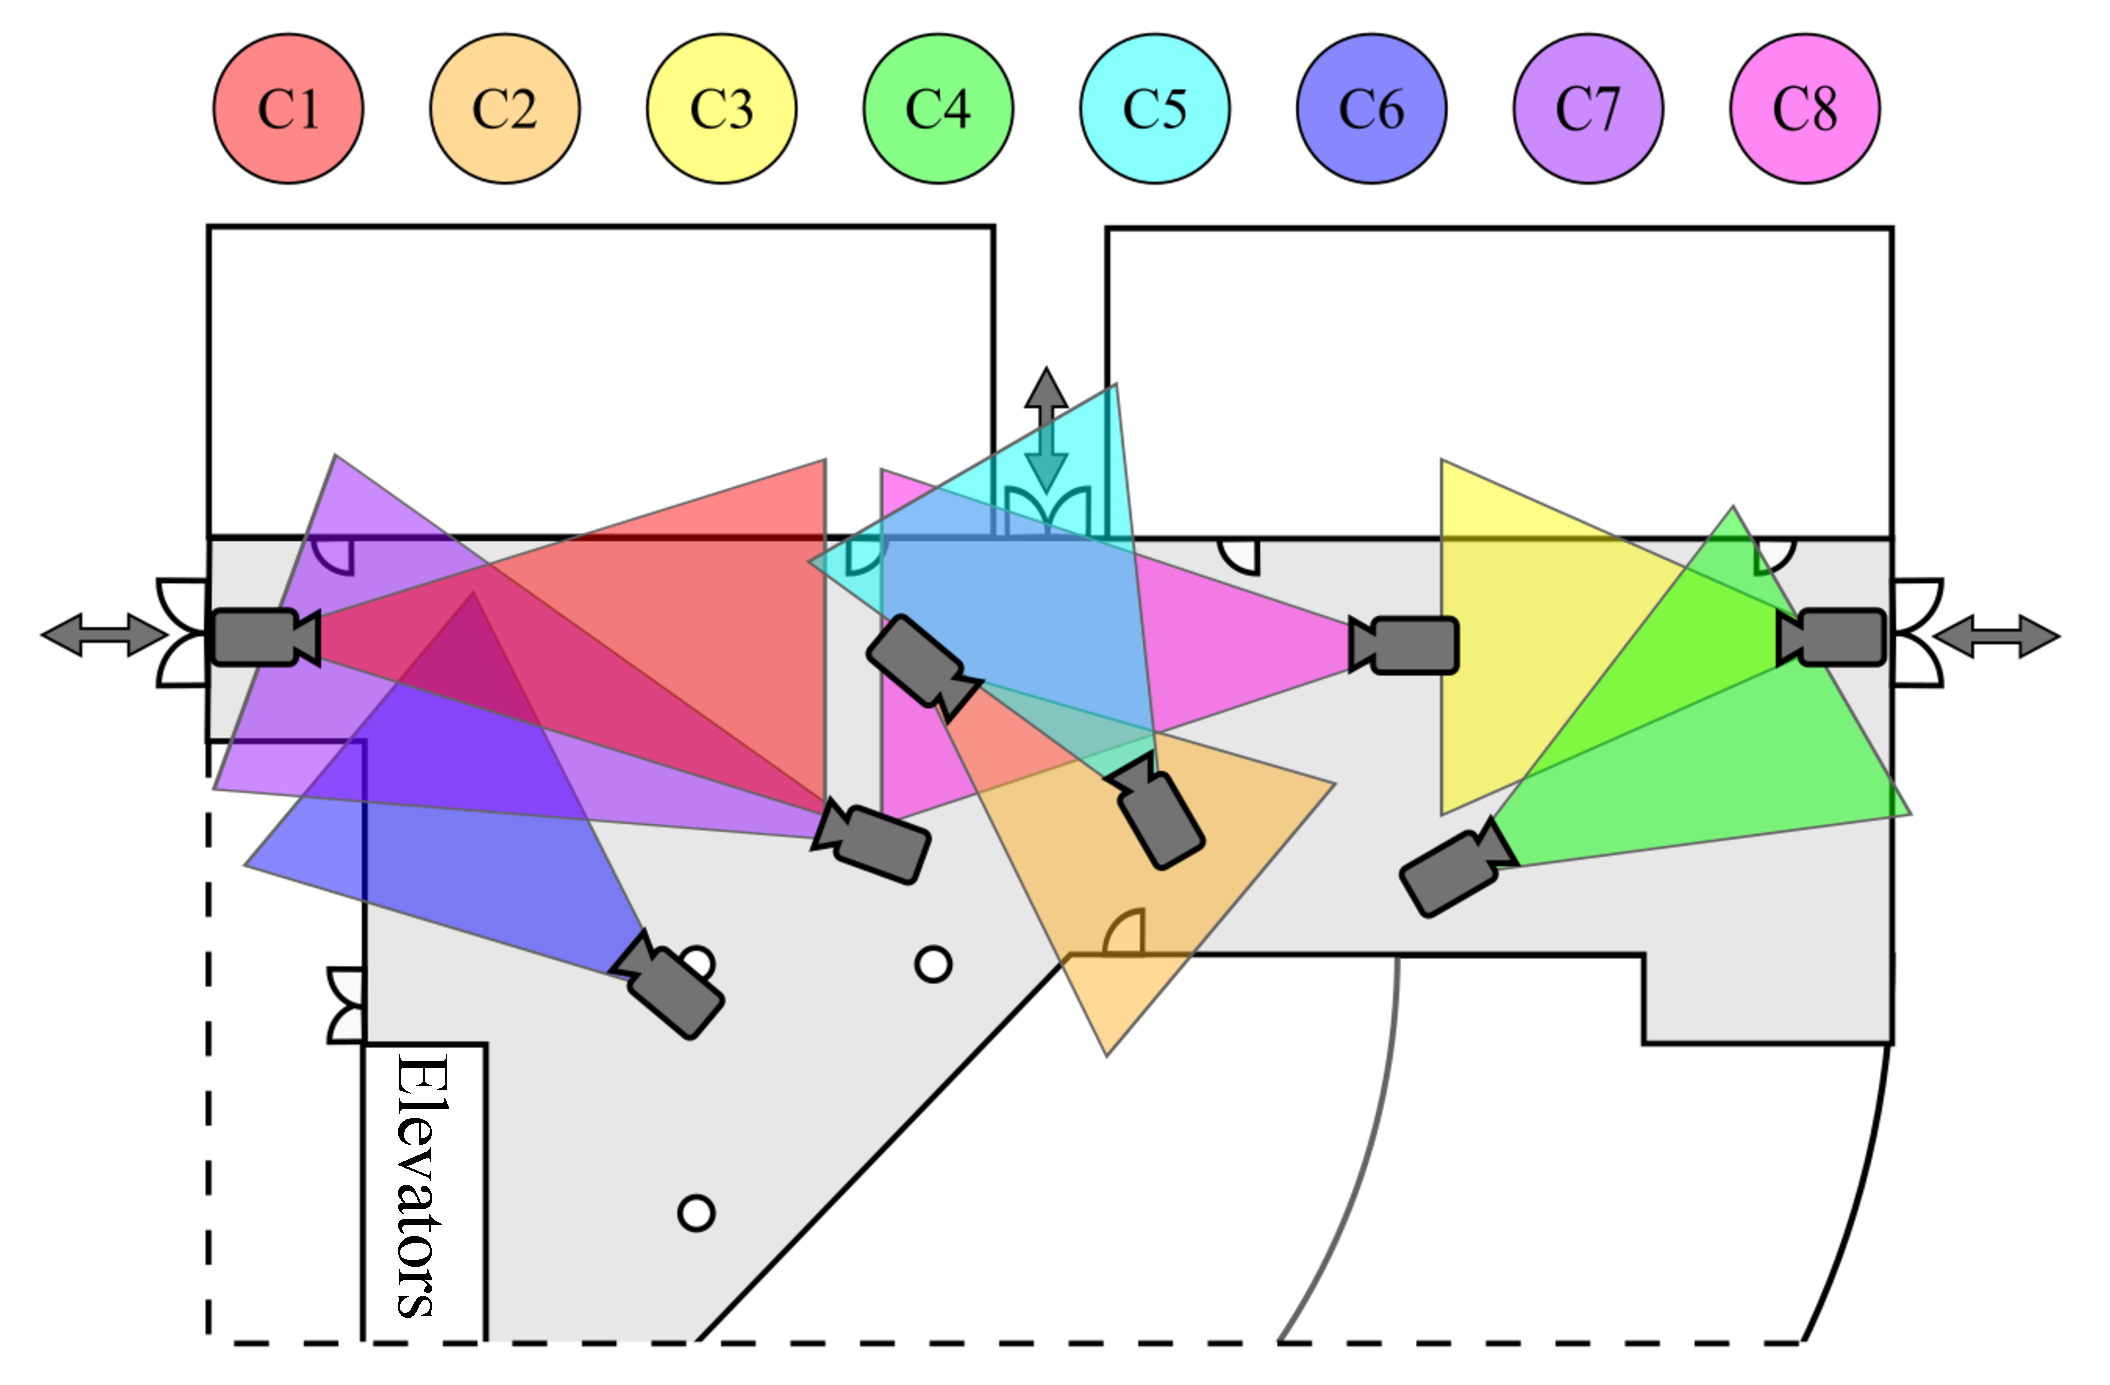
\includegraphics[width=0.7\textwidth]{figures/person_reid.eps}}
	\caption[A basic person re-identification scenario]
	{A basic person multi-camera person re-identification scenario. A person should have the same label when walking through the multiple surveillance camera network. \label{fig:person_reid}}
\end{figure}


\section{Gait Recognition}
\subsection{Context}
Biometrics refers to automatic identification or authentication of people by analyzing their physiological and behavioral characteristics. Physiological biometrics is related to the shape of body parts such as face, fingerprints, shape of the hand, iris, retina, etc., which are not subject to change due to aging. It is now used as the most stable means for authenticating and identifying people in a reliable way. However, for efficient and accurate authentication, these traits require cooperation from the subject along with a comprehensive controlled environmental setup. Hence, these traits are not useful in surveillance systems. Behavioral biometrics such as signatures, gestures, gait, and voice, etc., is related to a person’s behavior. But, these traits are more prone to change depending on factors such as aging, injuries, or even mood. 


\subsection{Definition}
Gait can be defined as \textit{the coordinated, cyclic combination of movements that result in human locomotion}~\cite{Boyd_05}. The movements in a gait repeat as a walker cycles between steps with alternating feet. It is both the coordinated and cyclic nature of the motion that makes gait a unique phenomenon.

Gait recognition is a behavioral biometric modality that identifies a person based on the gait pattern. In contrast to other biometrics such as face and fingerprint, it is a non-invasive technique for identifying an individual which is hard to copy. A unique advantage of gait as a biometric is that it offers recognition at a distance and at low-resolution images; consequently, gait biometric signature is now considered as the only likely identification technology suitable for access control, covert video surveillance, criminal investigation, and forensic analysis and the method is not vulnerable to spoofing attacks and signature forgery.


\subsection{Challenges}
Due to the advantages of gait recognition, the past two decades have witnessed significant improvements of its algorithms. However, unfortunately, there still exist many challenges that need to be addressed for robust gait recognition. It has been observed that the performance of gait recognition is highly affected by different intraclass variations in people's appearance such as clothing and carrying variation, and in environment such as variations in illumination, walking surface, and view angle, etc. These factors can drastically reduce the performance of gait recognition.  


\section{Problem Definition}
Gait based person re-identification in surveillance is a problem of recognizing individuals based on their gait pattern at different times and locations from a network of interconnected cameras, without overlapping views. The variation of people appearance and viewing angle at different cameras, varying lighting, and occlusion, however, make the problem very challenging. Although a multitude of researches have been done in recent years, it remains an open problem and many of its aspects have yet to be addressed.


\section{Objectives of the Thesis}
The objective of this thesis is to design a gait recognition system for human identification in a multi surveillance camera environment. To achieve this objective, we have identified the following specific aims.
\begin{itemize}
\item To design a novel low-dimensional gait feature descriptor based on the pose information of the people detected in the gait videos To design a mechanism to detect people in gait videos and determine their pose sequences. 
\item To develop a robust pose based gait recognition algorithm using recurrent neural network (RNN), which will be invariant to factors like viewing angle, clothing, presence of bags, etc.
\item To identify people across a set of interconnected surveillance cameras.
\item To compare the results with state-of-the-art methods.
\end{itemize}



\section{Overview of the Thesis}
Modern deep learning-based algorithms have recently gained increasing popularity while achieving outstanding performance in many computer vision tasks like video classification~\cite{karpathy_14}, pose estimation~\cite{Cao_19}, and action recognition~\cite{Song_17, Du_15}, etc. Furthermore, advancement on human body pose estimation can significantly assist in accurately modeling different body parts required for model-based gait recognition. On the other hand, recurrent neural networks \gls{rnn}s have also achieved a promising performance in many sequence labeling tasks. The reason behind their effectiveness for sequence-based tasks lies in their ability to capture long-range dependencies in a temporal context from sequence. \gls{rnn}s have been successfully employed to achieve state-of-the-art results in many vision-based tasks like human emotion detection and action recognition.

In this work, we propose a model-based gait recognition method where we consider human 2D pose data as our effective gait features. As body pose is proven not to depend on people body appearance and shape, and is invariant to change of clothing and carrying conditions. Additionally, as gait can be considered a time series of walking postures, body pose information has a powerful capacity to capture the temporal pattern of gait. Therefore, the proposed method will be less affected by the variation of covariate factors. It is also worth mentioning that, in this work we didn't use 3D pose data as our gait feature: firstly, computing 3D poses is computationally expensive, and secondly, most of the 3D pose estimation algorithms from 2D RGB images often require multiple views, and hence multiple cameras, rendering the technique unsuitable for surveillance. Again, recovering 3D pose from a single RGB images is an ill-posed problem and often causes large pose estimation errors. 

Compared to other gait covariate, view is the most important factor severely affecting gait recognition performance. To handle view variation efficiently, gait algorithms have generally been studied under three experimental setups: single-view, multi-view, and cross-view setup. In single-view gait recognition, both probe and gallery gaits are kept within same view angle, where in cross-view gait recognition, the probe and gallery gaits are kept in different views; and in multi-view gait recognition, multiple views of gallery gaits are combined to recognize a probe gait under a specific view.

Thus, the key to our proposed method is to develop a pose-based recurrent neural network for robust gait recognition by modeling the temporal dynamics associated with human gait. Most of the descriptors proposed in the literature for gait recognition often lead to a high dimensional feature space, which can be computationally expensive to map. In this work, we designed a lower dimensional spatio-temporal feature descriptor from 2D pose estimation for improved performance at a reduced computational cost. Our gait descriptor is a concatenation of four different kinds of features which are robust to view variation. We demonstrate the effectiveness of our proposed method through extensive experiments on two public benchmark datasets:  the CASIA A and CASIA B gait dataset~\cite{Yu_06}. Our method achieved state-of-the-art performance on these two challenging gait datasets in both single-view and cross-view recognition, providing better results as compared to other methods proposed in the literature.

For multi-view gait recognition, we also propose a two-stage network in which we first determine the walking direction, i.e. the viewpoint angle of the camera using a 3D convolutional network and later identify the subject using proposed \gls{rnn} based temporal network trained on that particular angle. Our proposed two-staged network is far simpler and efficient in terms of time and space while outperforming present state-of-the-art networks on multi-view gait recognition.


\section{Contributions}
In summary the contributions of this thesis are fourfold:
\begin{itemize}
\item We propose a novel \gls{rnn} network with \gls{gru} architecture and devise several strategies to effectively train the network for robust gait recognition. 

\item We also propose a two-stage network for multi-view gait recognition in which we first identify the walking direction using a 3D convolutional network and then performs subject recognition using a temporal network trained on that particular angle.

\item The proposed pose-based \gls{rnn} network achieves the best results on two challenging benchmark datasets CASIA A and CASIA B by outperforming other prevailing methods in single-view and multi-view gait recognition at a significant margin.

\item We consider 2D coordinates of body pose to design a novel low-dimensional gait feature descriptor which is invariant to covariate factors and achieved comparable performance to the methods which require to calculate gait energy image (GEI) or expensive 3D poses for gait descriptors.
\end{itemize}


\section{Thesis Outline} 
In the rest of this thesis, we present the details of our approach to human identification based on robust gait recognition. Here
\begin{itemize}
\item \textbf{Chapter~\ref{ch:literature_review}} reviews the existing literature gait recognition and basic concepts of recurrent neural network, focused on their use in our models. 

\item \textbf{Chapter~\ref{ch:methodology}} describes our proposed network along with the steps regarding features extraction, preprocessing and network architecture for both single-view and multi-view gait recognition.. It also presents learning strategies of these models. 

\item \textbf{Chapter~\ref{ch:result_discussion} }gives the experimental evaluation of the proposed framework on publicly available datasets, namely CASIA A and CASIA B dataset. It also compare our results with other state-of-the gait recognition algorithms in different experimental setup on these datasets and discusses them. 

\item \textbf{Chapter~\ref{ch:conclusion}} provides a conclusion and presents possible future directions.
\end{itemize}


